\chapter{The Standard Model and Its Future}\label{sec:theory}
In Section \ref{sec:introduction}, we introduced the few obstacles facing the SM: The existence of dark matter, baryon-antibaryon asymmetry, and the evidence of neutrino masses and mixing.
The SM Lagrangian, written as in formula \ref{eq:SM}, does not have particle fields that can explain those phenomena.
\begin{equation}
\label{eq:SM}
\mathcal{L}_{SM} = \mathcal{L}_{Higgs}+\mathcal{L}_{Gauge}+\mathcal{L}_{Kinetic}+\mathcal{L}_{Yukawa}
\end{equation}
\begin{align*}
\end{align*}

Since it can not be explained by any of the particles' fields in the SM, it requires the addition of new particles' fields or new terms in the current SM Lagrangian expression.
New terms in the SM Lagrangian entail new vertices in the Feynman diagram, which open the door for a new understanding of high energy physics.
However, if those observations did not exist, the SM is complete within its framework except for the naturalness problem.

The naturalness problem originates from the SM Higgs being a scalar particle.
The formula \ref{eq:SM} has three fields: boson, fermion, and scalar.
Quantum Field Theory (QFT), humanity's mathematical framework used for the SM, explains matter as an excited state of fermion fields derived from the canonical quantization of the SM Lagrangian's fermion fields.
%Also, QFT explains forces of the universe as the exchange of boson particles among the fermions, which can be derived from the fermion kinetic term of the SM Lagrangian.
The fermions' fields have chiral symmetry as demonstrated in the kinetic term of the SM Lagrangian in the formula \ref{eq:Lag1} and \ref{eq:Lagr1}.

\begin{equation}
\label{eq:Lag1}
	\mathcal{L}_{L_{kin}}  = \bar{L}*i\gamma^{\mu}D_{\mu}L+h.c.
\end{equation}
\begin{equation}
\label{eq:Lagr1}
	\mathcal{L}_{R_{kin}}  = \bar{u}*i\gamma^{\mu}D_{\mu}u+\bar{d}*i\gamma^{\mu}D_{\mu}d+h.c.
\end{equation}
, where Dirac matrices are summed up over Lorentz indices for Lorentz invariance. A lefthand fermion is a doublet for weak force interaction, and a right-hand fermion is a singlet separated by the up-type fermion (neutrinos for leptons) and down-type fermion (electrically charged leptons for leptons).
Since fermions with left-hand chirality behave differently from fermions with right-hand chirality,
the covariant derivatives are also different for left-hand kinetic term and right-hand kinetic terms, being defined in \ref{eq:covld} and in \ref{eq:covrd}.
\begin{equation}
\label{eq:covld}
	D_{\mu}  = i\partial_{\mu}-\frac{1}{2}g\tau*W_{\mu}-\frac{1}{2}g^{'}YB_{\mu} 
\end{equation}
\begin{equation}
\label{eq:covrd}
	D_{\mu}  = i\partial_{\mu}-\frac{1}{2}g^{'}YB_{\mu} 
\end{equation}
, where $\tau$ is isospin for SU(2) weak force, and g, W are couplings and fields for the weak theory. g' and B are respective variables for quantum electrodynamics (QED).
The equations above show that the left-hand fermions are separated from the right-hand fermions.


Likewise, the bosons' fields satisfy special QFT framework symmetries.
The boson satisfies the U(1), SU(2), or SU(3) gauge symmetry and is expressed in gauge terms as in formula \ref{eq:Lag2}.
\begin{equation}
\label{eq:Lag2}
	\mathcal{L}_{Gauge} = -\frac{1}{4}B_{\mu\nu}*B^{\mu\nu}-\frac{1}{4}W_{\mu\nu}^{\tau}*W^{\mu\nu}_{\tau}-\frac{1}{4}G_{\mu\nu}^{\alpha}*G^{\mu\nu}_{\alpha}.
\end{equation}
, where B, W, and G are QED, weak, quantum chromodynamics (QCD) fields, $\tau$, $\alpha$ are SU(2), SU(3) group indices, respectively.

These symmetries provide one significant advantage in QFT, renormalization.
QFT understands the observed mass of particles in terms of its bare mass and correction as in \ref{eq:ren}.
\begin{equation}
\label{eq:ren}
	m_{f}^{2}=m_{f,0}^{2}+\delta m_{f}^2.
\end{equation}
The chiral and gauge symmetries make a correction term to zero and protect fermion and boson fields from the radiative correction in the renormalization process.

Unlike fermions or gauge bosons, the scalar field of the Higgs boson is not protected by any symmetry. It is subject to large radiative corrections, especially from the top quark loop.
Thus, the necessary radiative corrections are enormous for the SM to be valid up to the Planck or Grand Unification Theory (GUT) scales of $10^{16}$ GeV.
One needs exorbitant fine-tuning to fit the Higgs mass at the observed value of 125GeV.
One of the most popular solutions to this problem is Supersymmetry (SUSY), which assigns chirality to the Higgs particle.
SUSY solves the fine-tuning problem, neutrino masses, and provides a candidate for DM.

Unfortunately, the LHC has found no significant excess over the SM background in their search for SUSY\cite{SUSY}.
Although the non-observation of supersymmetric partner particles does not invalidate SUSY, it makes it less attractive among the particle physics community.
Non-observation of superpartners, particularly the stop (scalar partner of the top quark), has pushed its mass beyond 1TeV.
It generates a "little hierarchy" problem, but an alternative "neutral naturalness" solution remains.

The top partners are not charged under the SM color group in the framework of neutral naturalness.
Because of being colorless, their production cross section is much smaller, and the present limits on the top partner particles are well below 1TeV.
Examples of neutral naturalness models are the Twin Higgs \cite{Chacko:2005pe},
Folded SUSY \cite{Burdman:2006tz}, and the Quirky Little Higgs \cite{Cai:2008au} models.
Theoretical models provide the possibility of neutral Long-Lived Particles (LLPs), which may be produced in the proton-proton
collisions of the LHC and decay back to SM particles far from the interaction point (IP).\cite{Craig:2015pha}
If the mirror QCD gluons form scalar glueballs, the SM Higgs boson can become a "Higgs Portal" between the SM and BSM mirror QCD scalar glueballs.
In the Mirror SM and Twin SM models, only the SM Higgs boson can interact with both SM QCD and mirror QCD particles as in figure \ref{fig:2HiggsPortal}.
\begin{figure}[h!]
  \caption{A cartoon display of Higgs Portal process}
  \label{fig:2HiggsPortal}
  \centering
  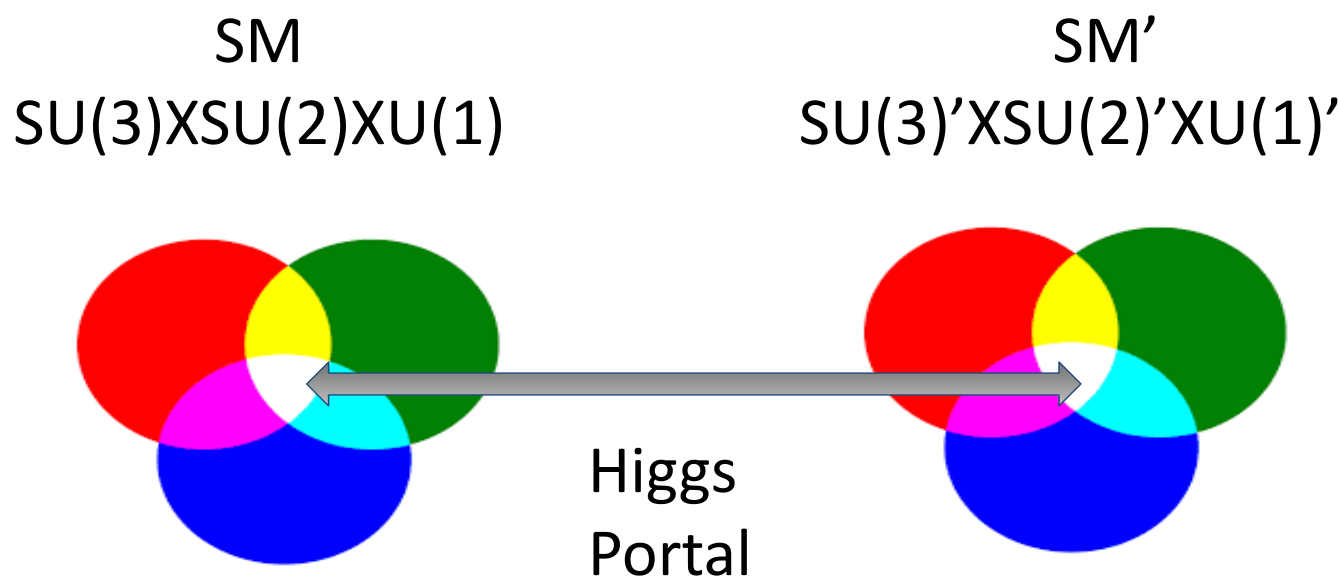
\includegraphics[width=0.87\linewidth]{figs/Portalcartoon.png}
\end{figure}
BSM mirror QCD scalar glueballs can only decay back to SM particles via Higgs boson decay.

Because of its decay as an off-shell Higgs boson, its cross section is highly suppressed.
The decay branching ratio to the highest mass fermions will be highest following the Yukawa couplings.
The decay ratio into b quarks or $\tau$ leptons is highest depending on the mirror scalar's mass.
However, if the Higgs has leptophilic behavior, the decay ratio into $\tau$ leptons is always the highest.
The displaced decays of the scalars would lead to exotic signatures in the CMS, such as distant innermost tracker hits, displaced vertices, and displaced jets.
The phenomenology of long-lived decay increased interest in a neutral naturalness among the particle physics community. \cite{Curtin:2015fna,Csaki:2015fba}.
The long-lived scalar model is shown in Figure \ref{fig:HiggsPortal}.



\begin{figure}[h!]
  \caption{A diagram display of Higgs Portal process}
  \label{fig:HiggsPortal}
  \centering
  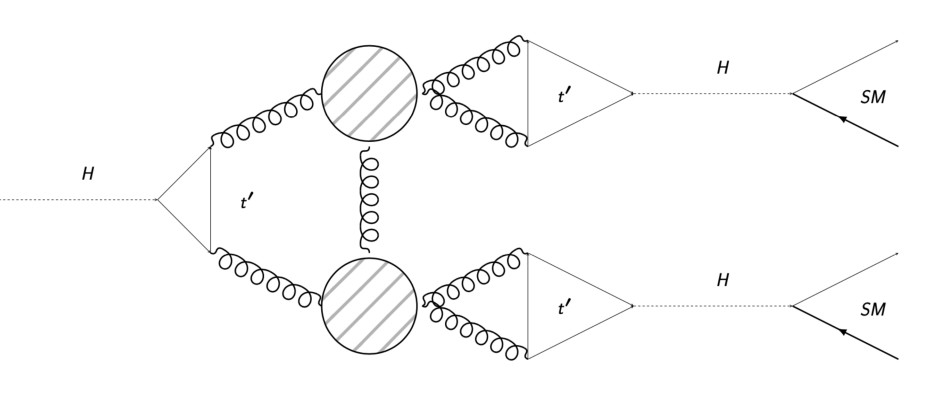
\includegraphics[width=0.87\linewidth]{figs/TwinHiggs.png}
\end{figure}
